
The first part of this Chapter describes details of the models from in Section~\ref{sec:monojet_scalar}, with 
emphasis on heavy flavour final states that arise due to the Yukawa couplings of SM quarks to the mediator. 
In addition, simplified models yielding signatures of a single top of bottom quark in the final state are outlined 
in Sections~\ref{sec:singletop, sec:singleb}. 
These models are not as generally applicable as those in the rest of this report, as they make a number of 
assumptions to enhance the production of these specific final states, but they are included as they still provide a 
unique search signature. Presentation of model-independent results is strongly encouraged to allow for further 
reinterpretation that relaxes some of the assumptions in these models.  

\section{\texorpdfstring{$t \bar{t}$ and $b \bar{b}$+MET models}{ttbar/bbar+MET models}}

\svnidlong
{$HeadURL$}
{$LastChangedDate$}
{$LastChangedRevision$}
{$LastChangedBy$}
\svnid{$Id$}

%As described in Section~\ref{sec:monojet_scalar}, a model with a scalar/pseudoscalar particle 
%mediating the DM-SM interactions is one of the simplest UV completions of our EFT models.  
With the MFV assumption, the top and bottom
quark can play an important  role in the phenomenology.
The scalar and pseudoscalar mediator models predict not only
the monojet process described in Section~\ref{sec:monojet_scalar}, but also production of Dark Matter
in association with top (or bottom) pairs, as illustrated in Fig.~\ref{fig:TTbarPhi}. 
Dedicated searches including jets from heavy flavor quarks in the final state
can be designed for this signature. Another class of simplified models,  
which includes a Dark Matter interpretation among many others, and yields a single
top quark in the final state, is detailed in Appendix~\ref{sec:singletop}. 

\begin{figure}[h!]
\centering
  \unitlength=0.005\textwidth
  \begin{feynmandiagram}[modelTTbarMET]
    \fmfleft{i1,i2}
    \fmfright{o1,o4,o5,o3}
    \fmf{gluon}{i1,v1}
    \fmf{gluon}{i2,v2}
    \fmf{fermion}{o1,v1,v3,v2,o3}
    \fmf{scalar}{v3,v4}
    \fmf{fermion}{o5,v4,o4}
    \fmf{phantom,tension=0,label={$\phi/a$}}{v3,v4}    
    \fmflabel{\Large $g$}{i1}
    \fmflabel{\Large $g$}{i2}
    \fmflabel{\Large $t (b)$}{o1}
    \fmflabel{\Large $\bar t (\bar b)$}{o3}
    \fmflabel{\Large $\chi$}{o4}
    \fmflabel{\Large $\bar \chi$}{o5}    
  \end{feynmandiagram}
%\caption[][\baselineskip]{Representative Feynman
\caption{Representative Feynman
diagram showing the pair production of Dark Matter particles in
association with $t\bar t$ (or $b\bar b$).}
\label{fig:TTbarPhi}
\setfloatalignment{t}
\end{figure}

%\section{Specific models involving $b-$ quarks in the final state}

In addition to the $t\bar t$+DM models illustrated in Fig.~\ref{fig:TTbarPhi}, 
some theoretically motivated scenario (e.g. for high $tan\beta$ in 2HDM in the pMSSM) 
privilege the coupling of \spinzero mediators to down generation quarks.
This assumption motivates the study of final states involving $b$-quarks 
as a complementary search to the $t\bar
t$+DM models, to directly probe the $b$-quark coupling. 
An example of such a model can be found in Ref.~\cite{Buckley:2014fba}
and can be obtained by replacing top quarks with $b$ quarks in Fig.~\ref{fig:TTbarPhi}.
Note that, because of the kinematics features of $b$ quark production relative
to heavy $t$ quark production, a $b\bar b$+DM final state may only yield one
experimentally visible $b$ quark, leading to a mono-$b$ signature in a model that conserves $b$ flavor.

Dedicated implementations of these models for the work of this Forum are available at LO+PS accuracy,
even though the state of the art is set to improve on a timescale beyond that for early Run-2 DM searches
as detailed in Section~\ref{sec:TTBar_implementation}.
The studies in this Section have been produced using a leading order UFO model within \madgraph 2.2.2
~\cite{Alwall:2014hca,Alloul:2013bka,Degrande:2011ua} 
using \pythiaEight for the parton shower. 

\subsubsection{Parameter scan}

%As discussed in Sec.~\ref{subsec:MonojetLikeModels}, the MFV and universal coupling assumptions for \spinzero
%mediators lead to quark mass dependent Yukawa couplings and therefore dominant couplings to top quarks.

The parameter scan for the dedicated $t\bar{t}$+\MET{} searches has been studied in detail to target the production 
mechanism of DM associated with heavy flavor quarks, and shares many details of the scan for the scalar model with a gluon radiation.
The benchmark points scanning the model parameters have been selected to ensure that the kinematic features of the 
parameter space are sufficiently represented. Detailed studies were performed to identify points in the \mdm, 
$m_{\phi,a}$, $\gDM$, $\gq$ (and $\Gamma_{\phi,a}$) parameter space that differ significantly from each other 
in terms of expected detector acceptance. Because missing transverse momentum is the key observable for searches, the 
mediator $p_{T}$ spectra is taken to represent the main kinematics of a model. Another consideration in determining the set 
of benchmarks is to focus on the parameter space where we expect the searches to be sensitive during the 2015 LHC run. 
Based on a projected integrated luminosity of $30\,{\rm fb}^{-1}$ expected for 2015, we disregard model points with a 
cross section times branching ratio smaller than $0.1\,{\rm fb}$, corresponding to a minimum of one expected event 
assuming a 0.1\% efficiency times acceptance. 

The kinematics is most dependent on the masses \mdm and $m_{\phi,a}$. Figure~\ref{fig:scanPhi} 
and~\ref{fig:scanPhiPseudo} show typical dependencies for scalar and pseudoscalar couplings respectively.
Typically, the mediator $p_T$ spectrum broadens with larger $m_{\phi,a}$. 
The kinematics are also different between on-shell ($\mMed>2\mdm$) and off-shell ($\mMed<2\mdm$) mediators as discussed in Section~\ref{sec:monojet_scalar}. 
Furthermore, the kinematic differences in the \MET{} spectrum between scalar and pseudoscalar are larger for light mediator 
masses with respect to heavier mediators. It is therefore important to  
choose benchmark points covering on-shell and off-shell mediators with sufficient granularity, including the
transition region between on-shell and off-shell mediators. %, as inFig.~\ref{fig:scanPhidiag}. 

\begin{figure}[!ht]
  \begin{center}
    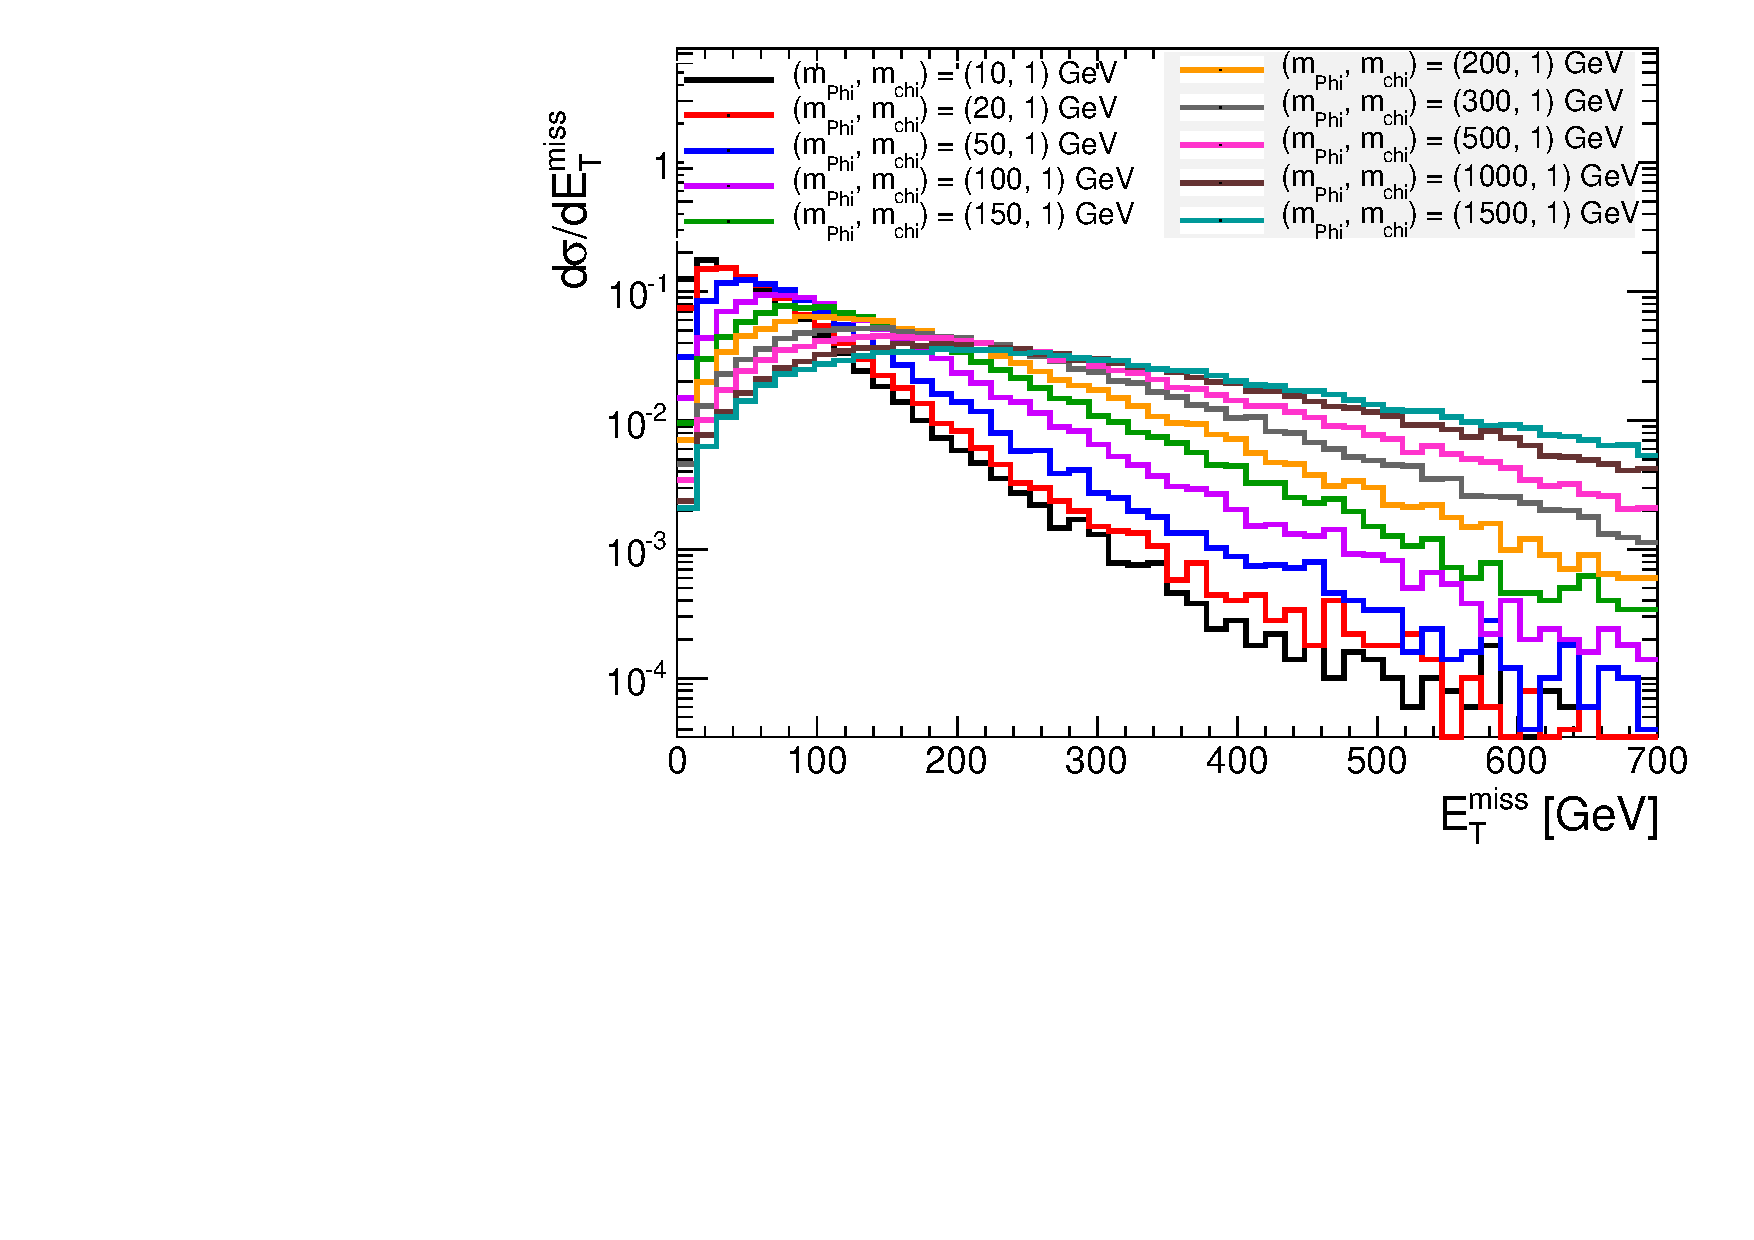
\includegraphics[width=0.95\textwidth]{figures/ttbar/MEt_chi1.pdf}
    \caption{\label{fig:scanPhi} Example of the dependence of the kinematics on the scalar mediator mass in the $t\bar{t}$+\MET{} signature. The Dark Matter mass is fixed to be \mdm=$1 {\rm GeV}$.}
\end{center}
\end{figure}


\begin{figure}[!ht]
  \begin{center}
    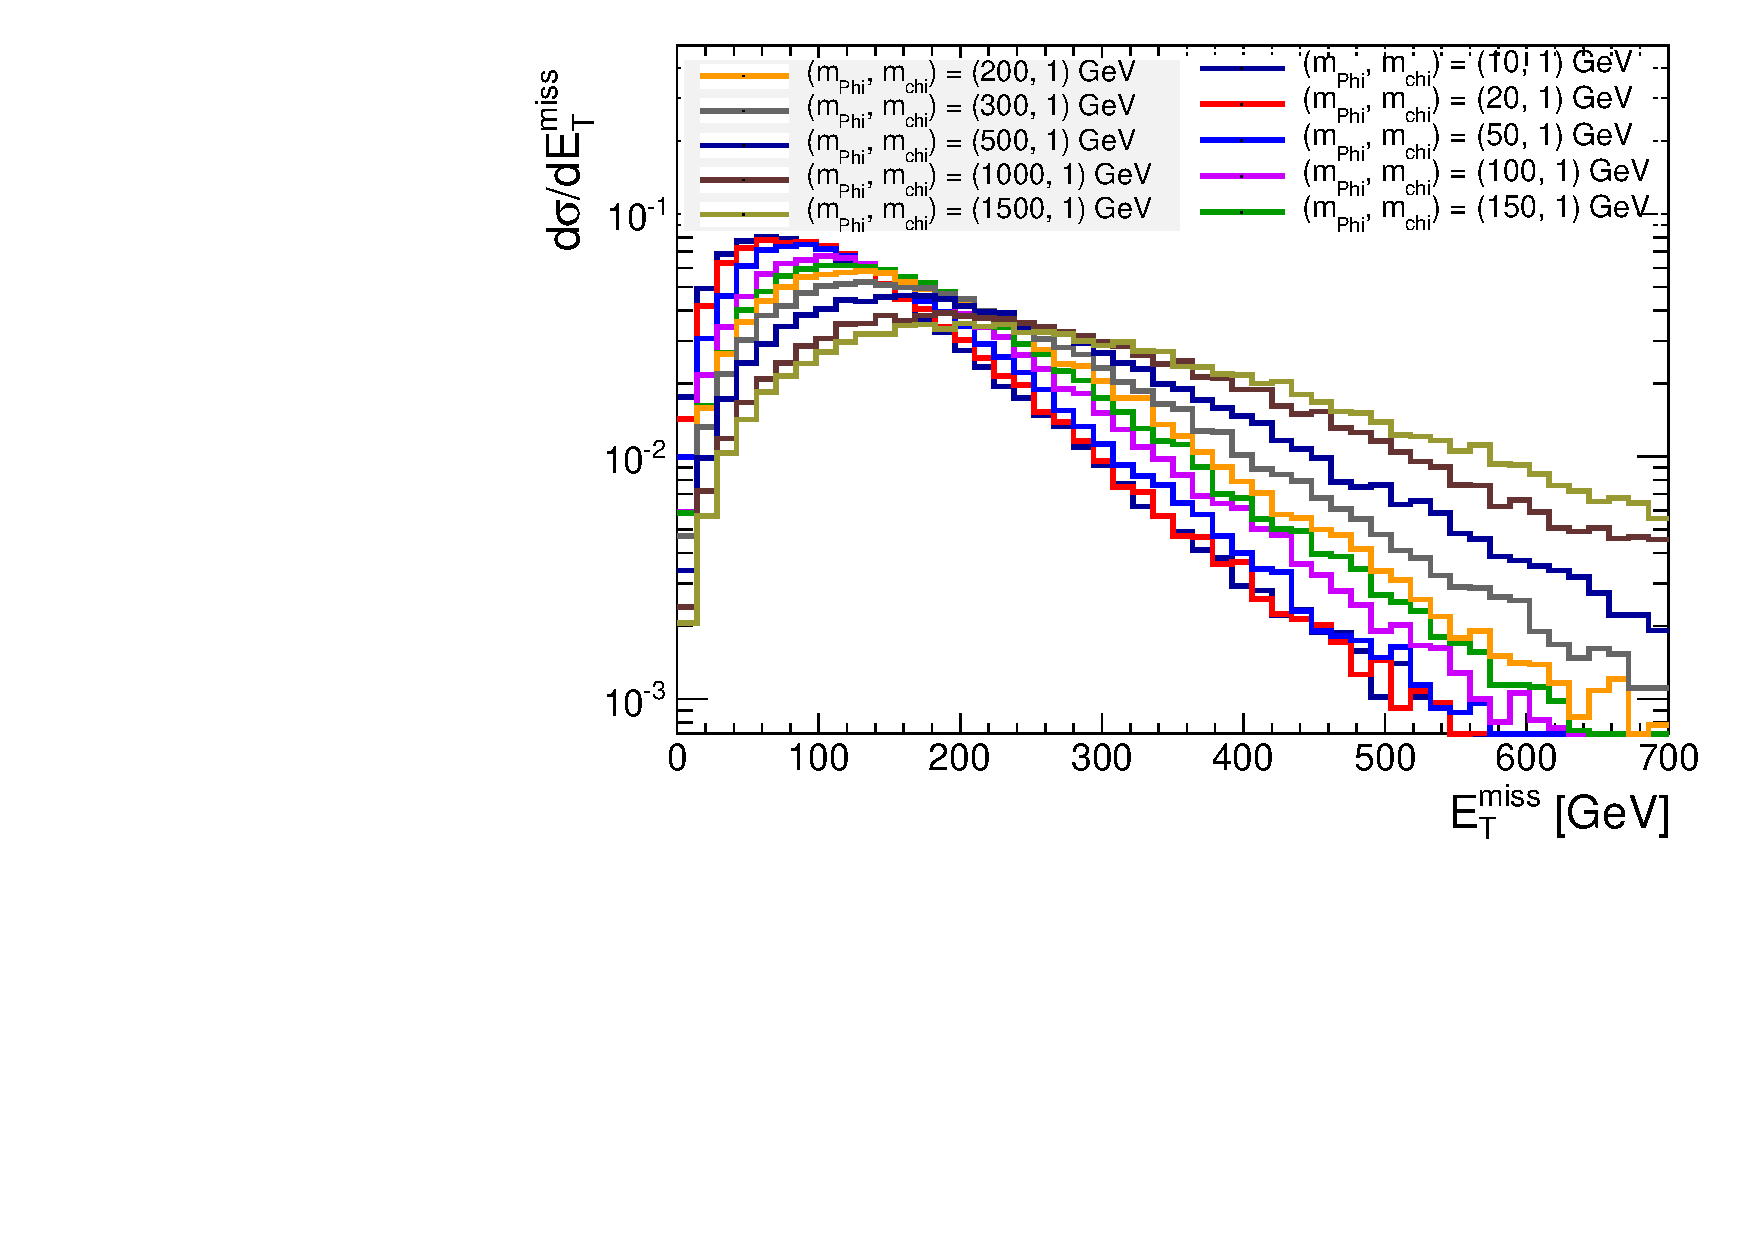
\includegraphics[width=0.95\textwidth]{figures/ttbar/MEt_chi1_pseudo.pdf}
    \caption{\label{fig:scanPhiPseudo} Example of the dependence of the kinematics on the pseudoscalar mediator mass in the $t\bar{t}$+\MET{}. The Dark Matter mass is fixed to be \mdm=$1 {\rm GeV}$. All figures concerning the $t\bar{t}$+\MET{}  signature have been produced using a leading order model within \madgraph 2.2.2, using \pythiaEight for the parton shower.}
\end{center}
\end{figure}

%\begin{figure}[!ht]
%  \begin{center}
%    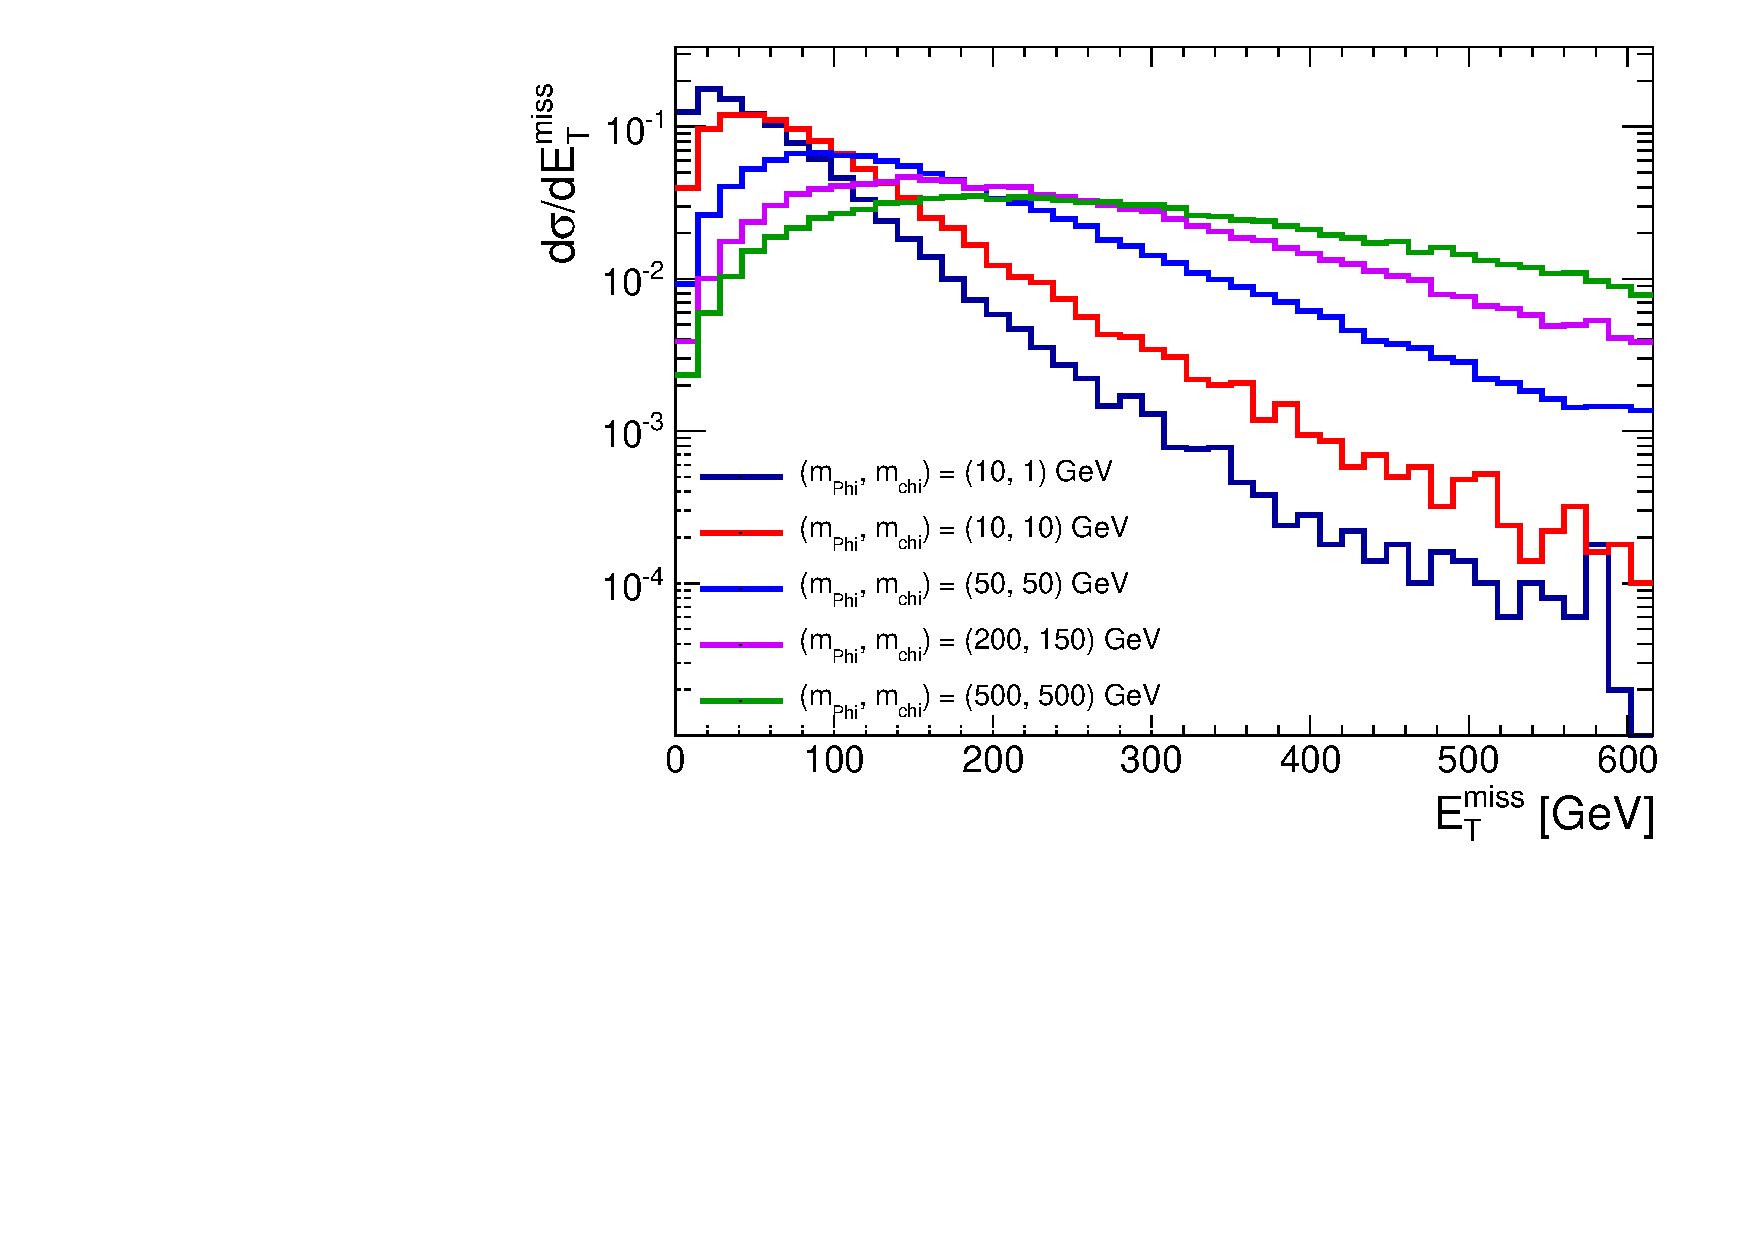
\includegraphics[width=0.95\textwidth]{figures/ttbar/MEt_diagonal_scan.pdf}
%    \caption{\label{fig:scanPhidiag} Example of the dependence of the kinematic for points of the grid proposed in Tab.~\ref{sec:monojet_scalar} close to the $m_{\phi,a} \sim 2m_\chi$ limit.
%    }
%\end{center}
%\end{figure}

Typically only weak dependencies on couplings are observed (see Fig~\ref{fig:widthsmallscan}) where the variation with width of the integral over parton distributions is unimportant. As shown in Section~\ref{sub:parameter_scan_monojet}, for couplings $\sim O(1)$ the width is large enough that the $p_T$ of the mediator is determined mainly by the PDF. 

At large mediator masses ($\sim 1.5\,{\rm TeV}$) or very small couplings ($\sim 10^{-2}$), width effects are significant, but these regimes have production cross sections that are too small to be relevant for $30\,{\rm fb}^{-1}$ and are not studied here. However, with the full Run~2 dataset, such models may be within reach. 

\begin{figure}[!ht]
  \begin{center}
    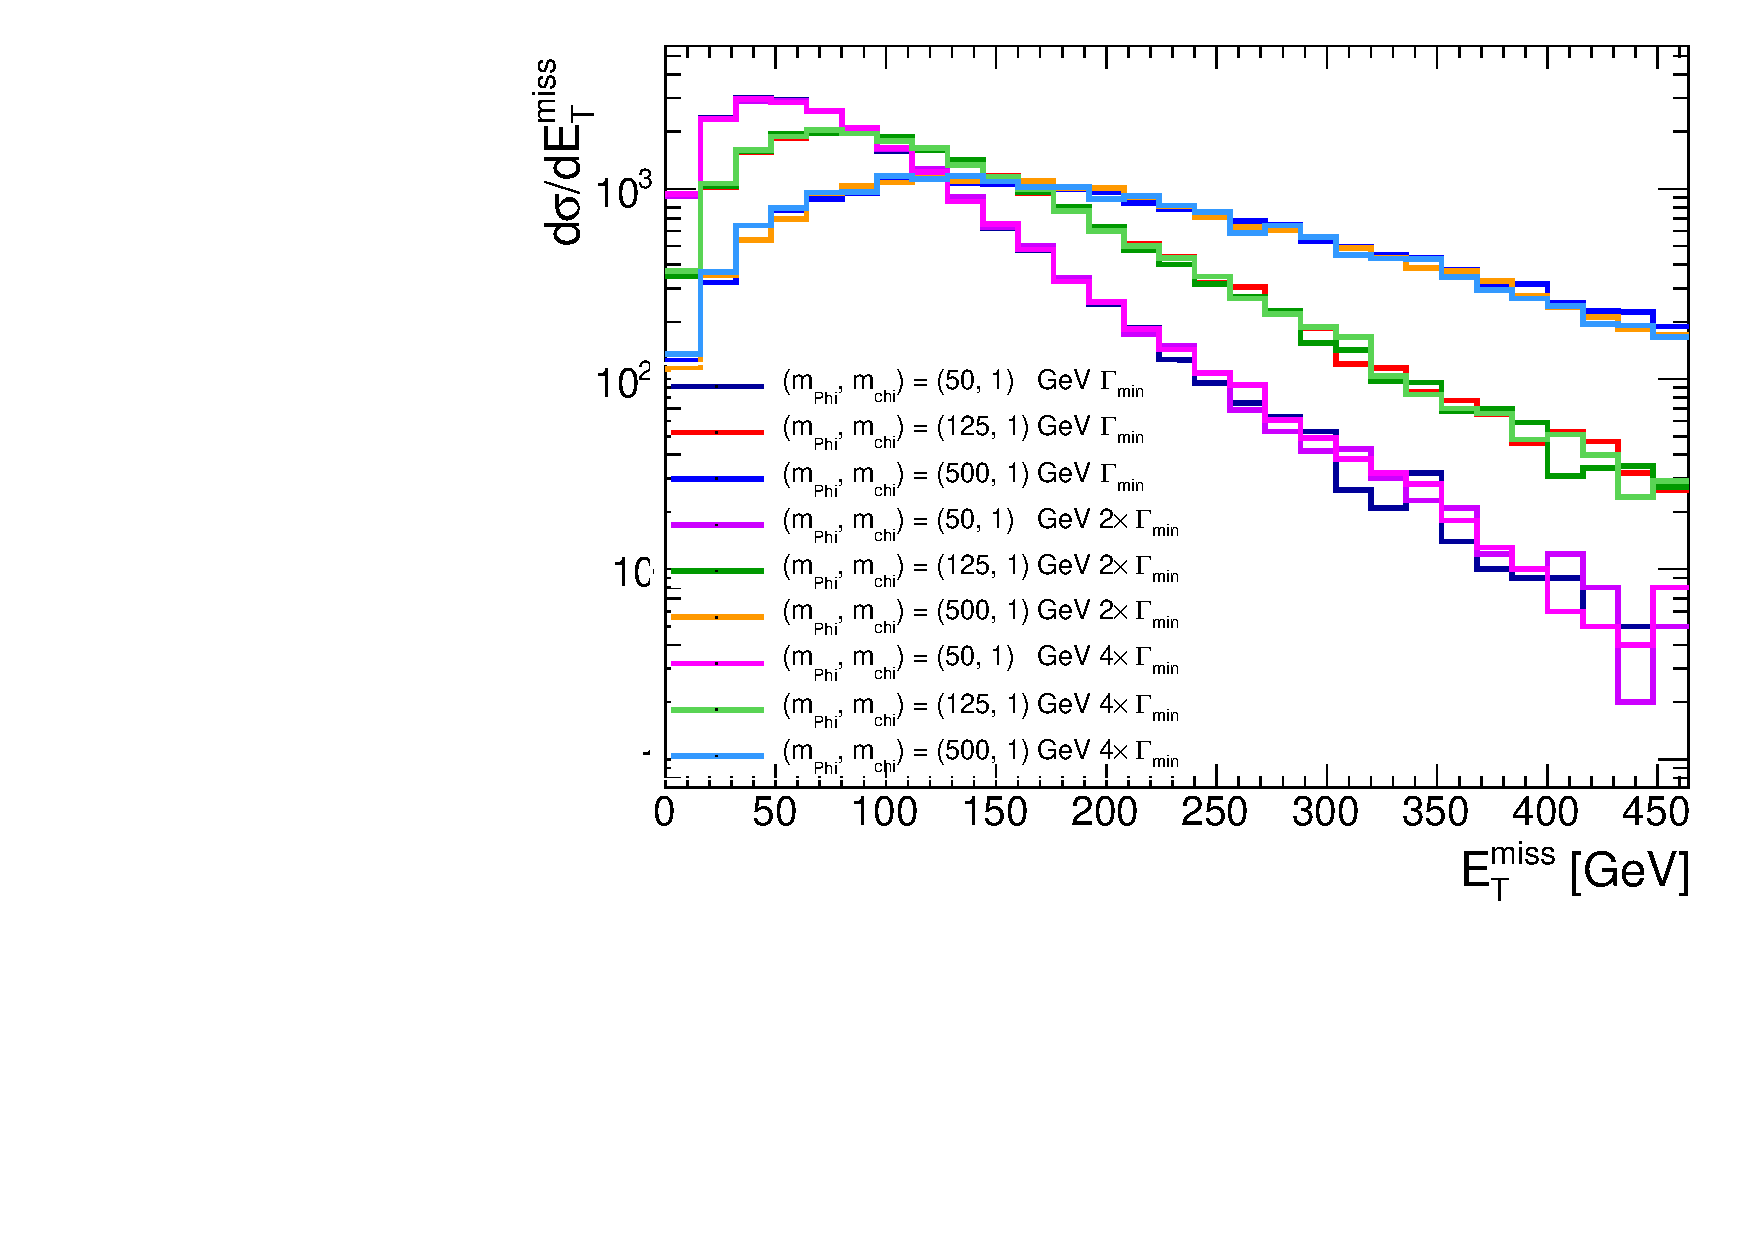
\includegraphics[width=0.95\textwidth]{figures/ttbar/MEt_smallwidth.pdf}
    \caption{\label{fig:widthsmallscan} Study of the dependence of kinematics on the width of a scalar mediator $t\bar{t}$+\MET{}. The width is increased up to four times the minimal width for each mediator and Dark Matter mass combination. 
    }
\end{center}
\end{figure}

Another case where the width can impact the kinematics is when $m_{\phi,a}$ is slightly larger than $2m_\chi$. Here, the width determines the relative contribution between on-shell and off-shell mediators. An example is given in Fig.~\ref{fig:widthlargescan}. As the minimal width choice pursued in this document is the most conservative one, this effect can be neglected in order to reduce the number of benchmark points to be generated. 

%In our recommendations we propose to use for simplicity the minimal width, as this is represents the most conservative choice to interpret the LHC results. 

\begin{figure}[!ht]
  \begin{center}
    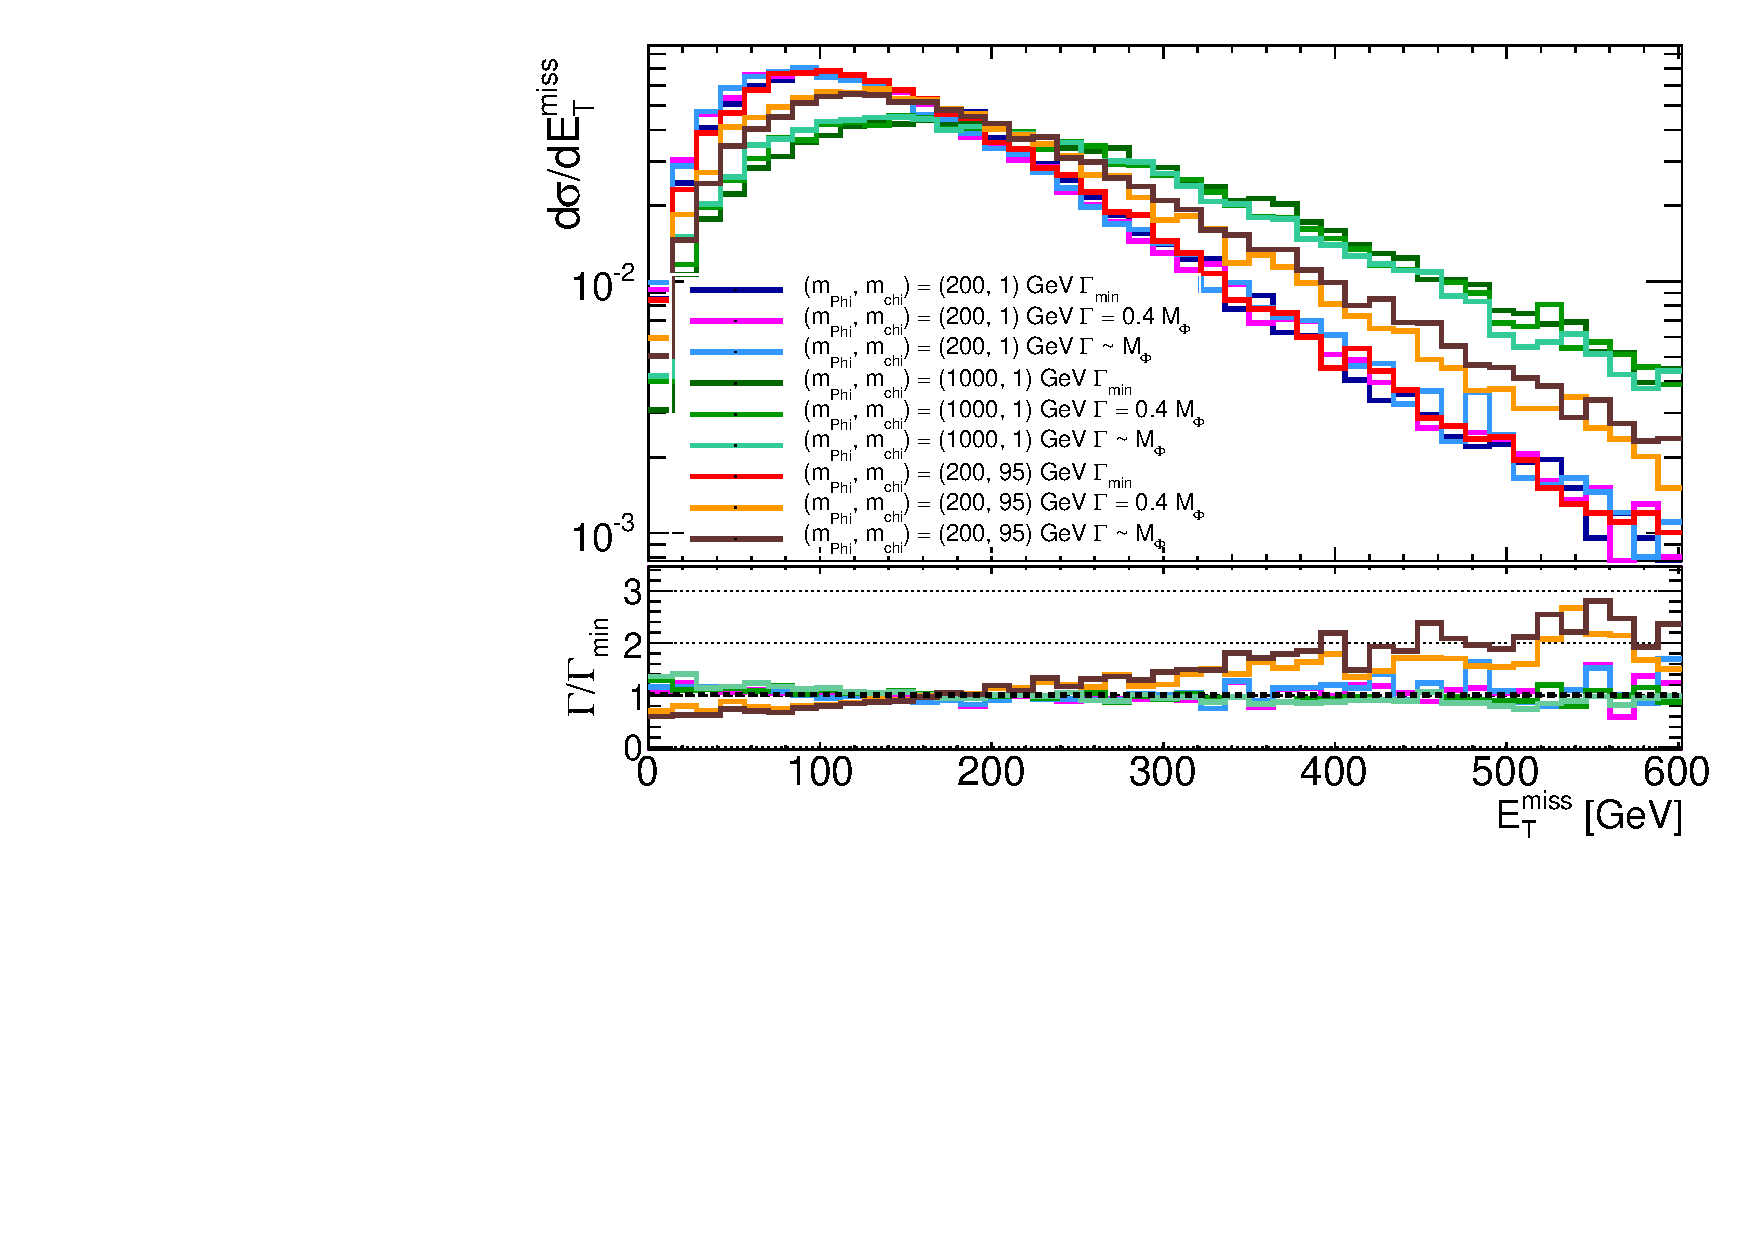
\includegraphics[width=0.95\textwidth]{figures/ttbar/ScalarWidth.pdf}
    \vspace{2mm}
    \caption{\label{fig:widthlargescan} Dependence of the kinematics on the width of a scalar mediator $t\bar{t}$+\MET{}. The width is increased up to the mediator mass. Choices of mediator and Dark Matter masses such that $m_{\phi,a}$ is slightly larger than $2m_\chi$ is the only case that shows a sizeable variation of the kinematics as a function of the width.  
    }
\end{center}
\end{figure}

The points for the parameter scan chosen for this model are listed in Table~\ref{tab:mDMmMedScan_SP}, chosen
to be harmonized with those for other analyses employing the same scalar model as benchmark. 
Based on the sensitivity considerations above, DM masses are only simulated up to 500 GeV (but the 5 TeV mediator point is retained)
leading to a total of 24 benchmark points. However for these searches we recommend to generate and simulate scalar and pseudoscalar
models separately, as the kinematics differs due to the different coupling of the mediator to the final state top quarks in the two cases,
as shown in Figs.~\ref{fig:scanPhi} and ~\ref{fig:scanPhiPseudo}.

Similar studies were performed in the $b \bar b$ case. It was found that they 
show the same weak dependence of the kinematics of the event on the mediator width.
The same benchmark parameters of the $t\bar t$ case could then be chosen.

%%
%[24/05/15 23:48:07] Caterina Doglioni: the plots are made with 5F, while we recommend 4F scheme
%[24/05/15 23:49:04] Caterina Doglioni: even though the relevant parameters do not change 
%(there are some plots due in the appendix for that, albeit with limited statistics), she doesn’t want to put them in 
%and wouldn’t be able to remake them with the right flavor scheme.

% Plots for bbar, if they make it
% Removing these plots as they won't make it last-minute. 
%\Todo{[TODO: The following figures are placeholders for now and will be added later].  If these are supporting material for the MC generation, put in the appendix}.
%
%\begin{figure}
%    \vbox{\hfill}
%    \caption{\label{fig:bbscanPhi} Example of the dependence of the kinematics on the scalar mediator mass. 
%    	The Dark Matter mass is fixed to be $1 {\rm GeV}$.}
%\end{figure}
%
%\begin{figure}[!ht]
%    \vbox{\hfill}
%    \caption{\label{fig:bbscanPhiPseudo} Example of the dependence of the kinematics on the pseudoscalar mediator mass. 
%    	The Dark Matter mass is fixed to be $1 {\rm GeV}$.}
%\end{figure}


%\newthought{Implementation}
%There are some subtleties to the Monte Carlo simulation relevant for
%this case that are discussed in Section~\ref{app:MonojetLikeModels_Appendix}.

%In addition to the considerations discussed in the preceding subsections, very light DM fermions are included ($\mdm=10\,{\rm GeV}$) 
%as this is a region where colliders have a complementary sensitivity to current direct detection experiments. 
% 
% \begin{table}[!ht]
% \centering
% \begin{tabular}{| l | r |}
% \hline
% \multicolumn{1}{|c|}{\mdm (${\rm GeV}$)} & \multicolumn{1}{c|}{$m_{\phi,a}$ (${\rm GeV}$)} \\
% \hline
%  $1$    & $10$, $20$, $50$, $100$, $150$, $200$, $300$, $500$, $1000$, $1500$  \\
%  $10$   & $10$, $20$, $50$, $100$, $150$, $200$, $300$, $500$, $1000$, $1500$  \\
%  $50$   &             $50$, $100$, $150$, $200$, $300$, $500$, $1000$, $1500$  \\
%  $150$  &                          $150$, $200$, $300$, $500$, $1000$, $1500$  \\
%  $500$  &                                               $500$, $1000$, $1500$  \\
% \hline
% \end{tabular}
% \caption{Simplified model benchmarks for $t\bar{t}$+DM production via \spinzero mediators decaying to Dirac DM fermions taking the minimum width presciption for $g_v = \gDM = 1$.}
% \label{tab:ttdm_benchmarks}
% \end{table}
% 


\section{\texorpdfstring{Models with a single $top-$quark + MET}{Models with a single top-quark + MET}}
\label{sec:singletop}
\svnidlong
{$HeadURL$}
{$LastChangedDate$}
{$LastChangedRevision$}
{$LastChangedBy$}
\svnid{$Id$}

Many different theories predict final states with a single top and associated missing 
transverse momentum (monotop), some of them including dark matter candidates. 
A simplified model encompassing the processes leading to this phenomenology is described in Refs.~\cite{AndreaFuksMaltoni,Agram:2013wda,Boucheneb:2014wza},
and is adopted as one of the benchmarks for Run 2 LHC searches. 

A dark matter candidate \DMParticle{} and a new particle $M$ (vector or scalar) 
are added to the SM, in a theory that respects the $\SUtwoUone$ symmetry 
and produces a single top quark in association with either the DM particle or a new particle
decaying invisibly. 

Within this model, two distinct processes can lead to monotop production:
\begin{itemize}
	\item resonant production, as shown in the diagram of Fig.~\ref{fig:feyn_prod} (a), where a scalar (S in the figure, $\varphi$ in the following) or vector ($X$) field are exchanged in the s-channel, and decay into the a spin 1/2 invisible DM candidate (called $f_{met}$ in the figure) and a top quark;
	\item non-resonant production, as shown in the diagrams of Fig.~~\ref{fig:feyn_prod} (b) and (c), where a flavor-changing interaction produces a top quark in association with a new colored scalar ($\Phi$) or vector ($V$). The new colored particles, called $v_{met}$ in the figure, decay invisibly, e.g. to a pair of DM particles. $v_{met}$ can also decay into a top quark and an up quark, leading to a same-sign top quark final state; a detailed study of the complementarity of this signature is beyond the scope of this Forum report.  
\end{itemize}

\begin{figure}[!h!tpd]
\centering
\unitlength=0.0046\textwidth
\subfloat[\label{subfig:S1}]{
  \begin{feynmandiagram}[modelS1]
    \fmfleft{i1,i2}
    \fmfright{o1,o2}
    \fmf{dashes,label={\Large $S$}}{v1,v2}
    \fmf{fermion}{i2,v1,i1}
    \fmf{fermion}{v2,o1}
    \fmf{plain,tension=0}{v2,o2}
    \fmf{wiggly}{v2,o2}
    \fmfdot{v1,v2}
    \fmflabel{\Large ${\bar{s}}$}{i1}
    \fmflabel{\Large ${d}$}{i2}
    \fmflabel{\Large ${t}$}{o1}
    \fmflabel{\Large ${f_{met}}$}{o2}
  \end{feynmandiagram}
}\\\vspace{\baselineskip}
\subfloat[\label{subfig:S4s}]{
  \begin{feynmandiagram}[modelS4s]
    \fmfleft{i1,i2}
    \fmfright{o1,o2}
    \fmf{fermion,label={\Large $u$}}{v1,v2}
    \fmf{gluon}{i2,v1}
    \fmf{fermion}{i1,v1}
    \fmf{wiggly}{v2,o2}
    \fmf{fermion}{v2,o1}
    \fmflabel{\Large $v_{met}$}{o2}
    \fmflabel{\Large $t$}{o1}
  \end{feynmandiagram}
}
\subfloat[\label{subfig:S4t}]{
  \begin{feynmandiagram}[modelS4t]
    \fmfleft{i1,i2}
    \fmfright{o1,o2}
    \fmf{fermion}{i2,vup}
    \fmflabel{\Large $u$}{i2}
    \fmf{gluon,label={\Large $g$}}{i1,vdown}
    \fmflabel{\Large $g$}{i1}
    \fmf{fermion}{vup,vdown}
    \fmf{fermion}{vdown,o1}
    \fmflabel{\Large $t$}{o1}
    \fmf{wiggly}{vup,o2}
    \fmflabel{\Large $v_{met}$}{o2}
  \end{feynmandiagram}
}
\caption
{
Feynman diagram of leading order processes leading to monotop events: production of
a coloured scalar resonance $S$ decaying into a top quark and a spin-$1/2$ fermion $f_{met}$ (a),
$s-$ (b) and $t$-channel (c) non resonant production of a top quark in association with
a spin-1 boson $v_{met}$.
%Feynman diagram of leading order processes leading to monotop events: resonant production of
%$t$ via resonant new particle $M$ decaying into a top quark and $\Xnew$, which is the dark matter fermion $\chi$ (left),
%and $s$ and $t$ channel non-resonant production of a top quark in association with $\Xnew$, which is the new particle $M$ (middle and right).
}
\label{fig:feyn_prod}
\end{figure}

In the following, resonant and non-resonant production are treated independently as separate benchmarks. 
Only the case of a scalar resonance is considered for the resonant model, while the case of vector resonances is left for future studies. 
%CD: why? the vector is better in "revisiting monotop"

\newthought{Resonant production}
\label{sec:ResonantProd}

In this case, a colored $2/3$-charged scalar ($\varphi^{\pm}$) is produced resonantly and decays into a top quark and a spin-$1/2$ invisible particle, $\chi$.  The dynamics of the new sector is described by the following Lagrangian:

\be\label{eq:lagrangianResonant}\bsp
\lag &=
%\lag_{\rm SM} + \lag_{\rm kin} 
%%
%+ 
\bigg[
%\phi \bar u \Big[a^0_{FC}\!+\!b^0_{FC} \gamma_5 \Big] u \!+\!
%V_\mu \bar u \gmu \Big[a^1_{FC} \!+\! b^1_{FC} \gamma_5 \Big] u  \\
%%
%&+ 
\varphi \bar d^c
\Big[a^q_{SR} + b^q_{SR} \gamma_5 \Big] d +
\varphi \bar u \Big[a^{1/2}_{SR} + b^{1/2}_{SR} \gamma_5 \Big] \chi
%
\\ &
+ X_\mu \bar d^c\gmu
\Big[a^q_{VR} + b^q_{VR} \gamma_5 \Big] d
%
+ X_\mu \bar u \gmu
\Big[a^{1/2}_{VR} + b^{1/2}_{VR} \gamma_5 \Big] \chi + 
{\rm h.c.} \bigg] 
\esp\ee

%\begin{eqnarray}
%\label{eq:lagrangianResonant}
%\mathcal{L} =  d^{C}_{i} \:  [ (g^{v}_{\phi d})^{ij} +  (g^{a}_{\phi d})^{ij} \gamma^{5} ] \: d_{j} \: \phi^{\pm}  +  u^{C}_{k}  [ (g^{v}_{u\chi})^{k} + (g^{a}_{u\chi})^{k} \gamma^{5} ] \: \chi \: \phi^{\pm}
%%%CD: problems with the original typesetting
%\end{eqnarray}

where $u$ ($d$) stands for any $up$-quark ($down$-quark), 
the index $S$ ($V$) stands for scalar (vector) field, and the index $q$ 
runs over the three quark generations. 

%The first term leads to the production of the new particle and the last term allows its decay into a $up$-quark 
%and a non interacting fermion (in particular to the top quark when $(g^{v/a}_{u\chi})^{k}$ 
%is sizable mainly for $k=3$).
%This model is then described by the masses of the new particle $m_{\phi}$ and the invisible 
%fermion $m_{\chi}$, and the coupling 
%$(g^{v/a}_{\phi d})^{ij}$ and $(g^{v/a}_{u\chi})^{k}$.

In the notation of~\cite{Agram:2013wda}, 
the couplings of the new colored fields to down-type quarks are
embedded into the $3\times 3$ matrices
$a^q_{\{S,V\}R}$ (scalar/vector couplings) and $b^q_{\{S,V\}R}$ (pseudoscalar/axial vector couplings)
while those to the DM candidate $\chi$ and one
single up-type quarks are given by the three-component vectors
$a^{1/2}_{\{S,V\}R}$ and $b^{1/2}_{\{S,V\}R}$
in flavor space. 

% 
% \com{Question/comment: in this resonant model, this is not so obvious to interpret $\phi_{\pm}$ as the new particle since there is a vertex $\phi-u-\chi$.
% It is somehow breaking the concept of having a dark sector weakly coupled to ordinary matter via a new particle.}
In the following, we only consider the model with a new colored scalar, as the requirement of invariance
under $SU(2)_L \times U(1)_Y$ would require the introduction of further particles in the case of a new colored vector~\cite{Boucheneb:2014wza}.
Note that the resulting model can be likened to the MSSM with
an RPV coupling between a top squark and fermions and an RPC coupling
between a top squark--top--neutralino.


\newthought{Non-Resonant production}
\label{sec:NonResonantProd}

For the non-resonant production, the top quark is produced in association with the new particle:
either a new scalar ($\phi$) or a new vector ($V$). For simplicity, we only consider the case of a vector new particle, as the scalar case would involve a mixing with the SM Higgs boson and therefore a larger parameter space. The Lagrangian describing the dynamics of the non-resonant case is: 
%%CD: Full explanation is below
% First, the new particle can be a scalar field interacting with the SM field and the dark matter
% candidate as described in this lagrangian:
% \begin{equation}
%  \label{eq:lagrangianNonResonantScalar}
% \mathcal{L} =  u^{C}_{i} \:  [ (g^{v}_{\phi u})^{ij} +  (g^{a}_{\phi u})^{ij}  \gamma^{5} ] \: u_{j} \: \phi  
%  +  \chi^{C}  [ g^{v}_{\phi\chi} + g^{a}_{\phi\chi}  \gamma^{5} ] \chi \: \phi
% \end{equation}
% where $u$ stands for any $up$-quark, the index $v$ ($a$) stands for vectorial (axial), 
% $C$ means charge conjugate and $i,j,k$ run over the generations.
% The first term describes the interaction between the new particle and the $up$-quarks while the 
% second term leads to the decay of the new particle into invisible fermions. 
% In this model, there is necessarily a mixing between $\phi$ and  the Higgs boson field. 
% Additional parameters are then required to describe this new sector: in addition to 
% the new particle mass and couplings, the mixing matrix of the two scalar fields
% is needed in order to make predictions. For the sake of simplicity, 
% we do not consider this case were the parameters space would be too large.
\be\label{eq:lagrangianNonResonantVector}\bsp
\lag &=
%\lag_{\rm SM} + \lag_{\rm kin} 
%%
%+ 
\bigg[
\phi \bar u \Big[a^0_{FC}\!+\!b^0_{FC} \gamma_5 \Big] u \!+\!
V_\mu \bar u \gmu \Big[a^1_{FC} \!+\! b^1_{FC} \gamma_5 \Big] u  
%
%%&+ 
%\varphi \bar d^c
%\Big[a^q_{SR} + b^q_{SR} \gamma_5 \Big] d +
%\varphi \bar u \Big[a^{1/2}_{SR} + b^{1/2}_{SR} \gamma_5 \Big] \chi
%%
%\\ &
%+ X_\mu \bar d^c\gmu
%\Big[a^q_{VR} + b^q_{VR} \gamma_5 \Big] d
%%
%+ X_\mu \bar u \gmu
%\Big[a^{1/2}_{VR} + b^{1/2}_{VR} \gamma_5 \Big] \chi + 
+ \rm h.c. 
\bigg] 
\esp\ee

The strength of the interactions among these two states and a pair
of up-type quarks is modeled via two $3\times 3$
matrices in flavor space $a^{\{0,1\}}_{FC}$ for the scalar/vector couplings
and $b^{\{0,1\}}_{FC}$ for the pseudoscalar/axial vector couplings.

%The dynamics of this case is described by the following Lagrangian:
%\begin{equation}
% \label{eq:lagrangianNonResonantVector}
%  \mathcal{L}  =  \bar{u}_{i} [ (g^{v}_{Vu})^{ij} \gamma^{\mu} + (g^{a}_{Vu})^{ij} \gamma^{5} ] u_{j} \: V_{\mu}  
%  +  \bar{\chi} [ g^{v}_{Vu} \gamma^{\mu} + g^{a}_{V\chi} \gamma^{5} ]   \chi \: V_{\mu}
%\end{equation}
%where $u$ stands for any $up$-quark, the index $v$ ($a$) stands for vectorial (axial) and $i,j,k$ run over the generations.
%The first term describes the interaction between the new particle and the $up$-quarks while the second term leads to the decay the new particle 
%into invisible fermions. The new sector can be defined with the couplings $(g^{v/a}_{Vu})^{ij}$, 
%$g^{a/v}_{V\chi}$ and the masses $m_V$ and $m_{\chi}$. 
%This model can be probed by two different experimental signatures: monotop and same-sign top quark production. 
%% 
%% \com{Question for theorists: why it cannot mix with $\Zboson$ in case of vectorial new particle ?}

\newthought{Model parameters and assumptions}
 
The models considered as benchmarks for the first LHC searches
contain further assumptions in terms of the flavour and chiral structure of the model
with respect to the full Lagrangians of equations~\eqref{eq:lagrangianResonant} and~\eqref{eq:lagrangianNonResonantVector}.
These assumptions are qualitatively discussed below. 

\paragraph{Assumptions in the flavour and chiral structure of the models}

We only consider right-handed quark components, in order to simplify the model phenomenology. 
The representation of the left-handed components under the $\SUtwo$ symmetry would lead to a 
coupling to $down$-type quarks, since the effective theory is invariant under $\SUtwoUone$ 
gauge symmetry. Having a coupling between the new particle and $down$-type quarks 
would complicate the collider phenomenology, adding the
$V \to b\bar{d} + \bar{b}d$ decay mode in addition to the invisible decay mode. 
This in turn sets the scalar (vector) and pseudoscalar (axial vector) matrices to have 
elements of equal values. 

Furthermore, in order to be visible at the LHC in the monotop final state, 
these models must include a strong coupling between the new particle $\phi$ and $t\chi$.
%In the resonant case, the new particle must also couple to light quarks in order
%to be produced at the LHC, leading to possible constraints from
%dijet searches. 
The same kind of assumption exists for the non-resonant production. 
This means that only the couplings between the new scalar resonance and  
light quarks ($a_{VR}, a_{SR}$), and the couplings between the new vector, the top quark 
and light quarks ($a_{FC}$), are set to non-zero values 

\be\label{eq:a}\bsp
%& (a^0_{FC})_{13} = (a^0_{FC})_{31} = a
%}%% (a^1_{FC})_{13} = (a^1_{FC})_{31} = a \ , \\
%% &  (a^q_{SR})_{12} = \ -(a^q_{SR})_{21} = (a^{1/2}_{SR})_3 =
& (a^q_{VR})_{11} = (a^{1/2}_{VR})_3 = a
\esp 
\ee

%  (on top of $V \to t\bar{u} + \bar{t}u$ and $V \to \chi\chi$). 
 
%
%Typically, including 
%the left-handed components of quarks in the lagrangian~\eqref{eq:lagrangianNonResonantVector} 
%describing the $Vtu$ vertex would lead to 
%\begin{equation}
%\mathcal{L}_{Vtu} \; = \;  g^{R}_{Vtu} \: \bar{t}_{R}\gamma^{\mu}u_R \: V_{\mu} \; + \; g^{L}_{Vtu} 
%(\bar{t}_{L}\gamma^{\mu}u_L \: + \:  \bar{b}_{L}\gamma^{\mu}d_L ) \: V_{\mu}
%\end{equation}
%where $g^{R/L} \equiv 1/2 \, (g^{v} \pm g^{a})$ couples only to right-handed/left-handed components. 
%The second term stems from invariance under $\SUtwo$ rotations, and leads to an additional 
%decay mode $V \to b\bar{d} + \bar{b}d$ (on top of $V \to t\bar{u} + \bar{t}u$ and $V \to \chi\chi$). 

%Given that the new particle must be produced from a light quark in the initial state, 
%in association with a top quark, the monotop signature can mainly probe a high 
%coupling $\left(g^{v/a}_{Vu}\right)^{13}_{Vu} \equiv g^{v/a}_{Vtu}$. 

%Therefore,
%the sensitivity to other flavour couplings is significantly lower, since $V$ would be 
%produced at a lower rate. 

%CD: not sure I understand?
% In addition, the new particle must decay into invisible particles
% to lead to the searched monotop final state. As a consequence, the sensitivity for 
% scenario where $\BR{V}{\chi\chi}\ll 100\%$ can be quite low. 
% To cope with this second limitation, a same-sign top quark final state 
% $gu \to tV(\to t\bar{u})$ is proposed to cover the cases where $V$ would decay
% into visible particles. This case is more likely as the $tV$ production rate increases, 
% and becomes then a key point to constraint this model in a consistent way.

% % \com{Questions for theorists:
% % \begin{itemize}
% %  \item How well these flavour assumptions are allowed by the other HEP data (proton decay life time, flavour physics, etc ...) ?
% %  \item MFV criteria ?
% % \end{itemize}
% % }
% 
% \subsubsection{Chiral structure}
% \label{sec:chiralstructure}


\newthought{Implementation}

This Section describes the notations used in the MadGraph model convention, 
in term of the ones introduced in the previous Section.

The Madgraph model~\cite{MGmodel} used for these benchmarks corresponds to the Lagrangian from~\cite{AndreaFuksMaltoni}. 
Each coupling constant of this model can be set via the parameter card and 
the blocks which are relevant for the two models used for the experimental searches are described below.
The relevant parameters in the MadGraph parameter cards, also expressed in the notation introduced in the 
previous Section, are as follows for the two models considered.

\begin{enumerate}

\item Resonant scalar model described by the Lagrangian~\eqref{eq:lagrangianResonant}
  \begin{itemize}
  \item \texttt{AQS} and \texttt{BQS}: $3\times 3$ matrices (flavour space) fixing the coupling of the scalar $\phi$ ($S$ stands for scalar) and $down$-type quarks ($Q$ stands for quarks), previously called $a/b_{SR}$.
  \item \texttt{A12S} and \texttt{B12S}: $3\times 1$ matrices (flavour space) fixing the coupling of the DM candidate $\chi$ (where $12$ stands for spin-$1/2$ fermion) and $up$-type quarks, previously called $a^{1/2}_{VR}$.
  \item particle names: the scalar $\phi^{\pm}$ is labeled $S$ and the fermion $\chi$ is $f_{met}$
  \end{itemize}  
  
\item Non-resonant vectorial model described by the Lagrangian~\eqref{eq:lagrangianNonResonantVector}
\begin{itemize}
\item \texttt{A1FC} and \texttt{B1FC}: $3\times 3$ matrices (flavour space) fixing the coupling of the vector $V$ ($1$ stands for vector) and $up$-type quarks, previously called $a^0_{FC}$. 
\item particle name: the vector $V$ is labelled $v_{met}$, while the dark matter candidate $\chi$ is not implemented (as this model assumes $\BR{V}{\chi\chi}=100\%$)
\end{itemize}

\end{enumerate}

The width of the scalar resonance and of the new vector are set to only the allowed decays in the models,
namely a DM candidate and a top quark for the resonant model. 

%In the case of the non-resonant model and . 
%Further studies will show whether to a top and an up quark 

%The two matrices $A$ and $B$ are taken to be equal according to the chiral assumptions made above. 
%The convention adopted follows \cite{ATLASmonotop} in defining 
%a single number $a_{\mathrm{res}}$ ($a_{\mathrm{non-res}}$) 
%for the resonant (non resonant) model, such as $(\ares^q)_{\mathrm{12}}=(\ares^q)_{\mathrm{21}}=(\ares^{1/2})_{\mathrm{3}}\equiv \ares$ 
%(in order to have $d-s-S$ couplings, and $t-S-f_{met}$ couplings) 
%and $(\anonres)_{\mathrm{13}}=(\anonres)_{\mathrm{31}}\equiv \anonres$ (in order to have $v_{met}-t-u$ couplings). 

\newthought{Parameter scan}

The relevant parameters for the resonant model are:
\begin{itemize}
	\item The mass of the new scalar $\phi$;
	\item The mass of the DM candidate $\chi$;
	\item The coupling of the new scalar to the DM candidate and top quark $a$, 
	related to the width of the scalar in the minimal width assumption;
\end{itemize}	

The relevant parameters for the non-resonant model are:
\begin{itemize}
	\item The mass of the new vector $V$;
	\item The mass of the DM candidate $\chi$;
	\item The coupling of the new vector to the up and top quark $a$, 
	related to the width of the scalar in the minimal width assumption;
	\item The coupling of the new vector to the DM candidate $\chi$, 
	related to the branching fraction of the vector into invisible and visible particle,
	and as a consequence to the width of the vector. 
\end{itemize}	

It has been checked for the non-resonant model that the relevant kinematics does not change when changing the width of the resonance. Figures~\ref{fig:appB:Vmass}, \ref{fig:appB:pTV} and~\ref{fig:appB:pTtop} show the $V$ mass distribution, the transverse momentum for $V$ and for the top quark from the $V\to t\bar{u}$ decay, for different $V$ masses and widths.
These figures are relevant independently of the $V$ decay mode (be it visible or invisible). 

\begin{figure}[!h!tpd]
	\centering
	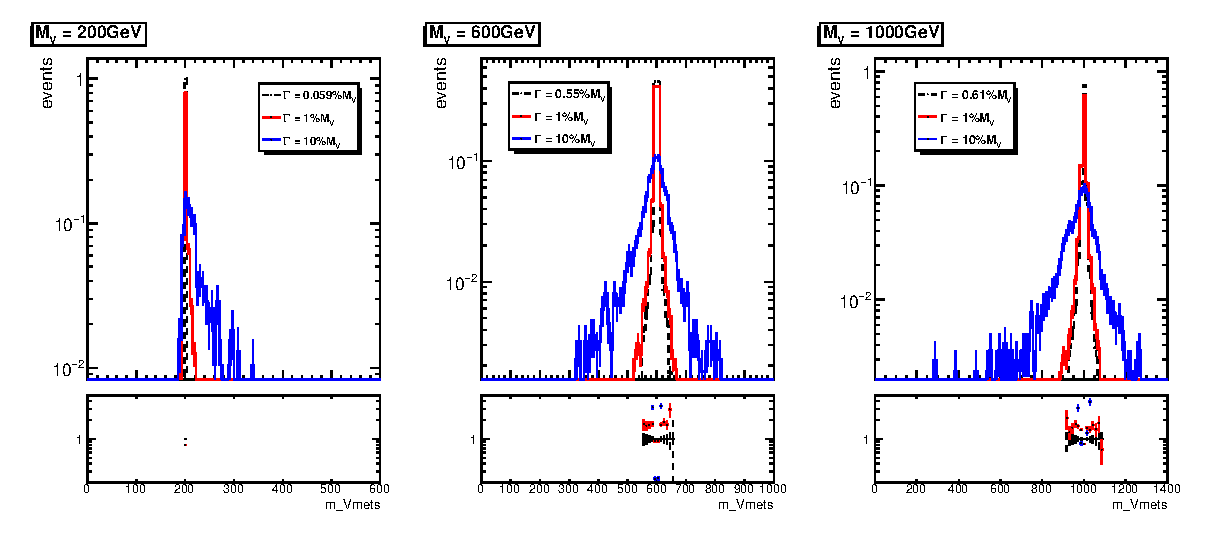
\includegraphics[width=1.0\textwidth]{figures/singletop/m_Vmets}
	\caption{
		Distribution of $V$ invariant mass for the $gu\to tV(\to t\bar{u})$ (on-shell V) 
		for $m_V$ = {200, 600, 1000}~GeV (from left to right) and for three different
		visible decay width (computed from Madgraph directly according to the allowed decays and their couplings, $1\%$ and $10\%$).
	}   
	\label{fig:appB:Vmass}
\end{figure}


\begin{figure}[!h!tpd]
	\centering
	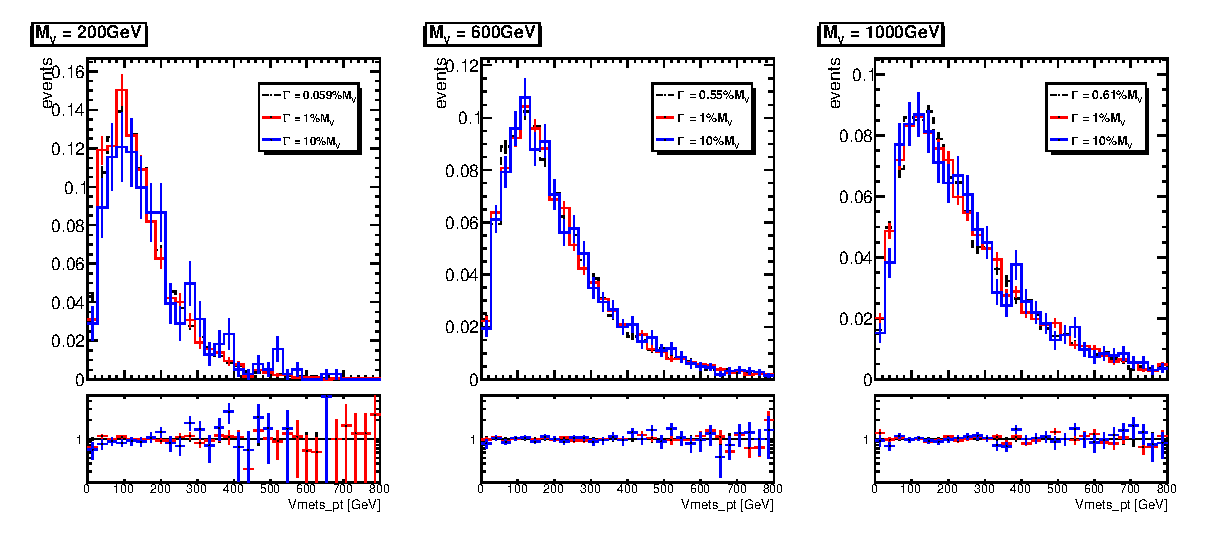
\includegraphics[width=1.0\textwidth]{figures/singletop/Vmets_pt}
	\caption{
		Distribution of the $V$ $p_T$ for the $gu\to tV(\to t\bar{u})$ (on-shell V) for $m_V$ = {200, 600, 1000}~GeV (from left to right) and for three different
		visible decay width (computed from Madgraph directly, $1\%$ and $10\%$).
	}
	\label{fig:appB:pTV}
\end{figure}


\begin{figure}[!h!tpd]
	\centering
	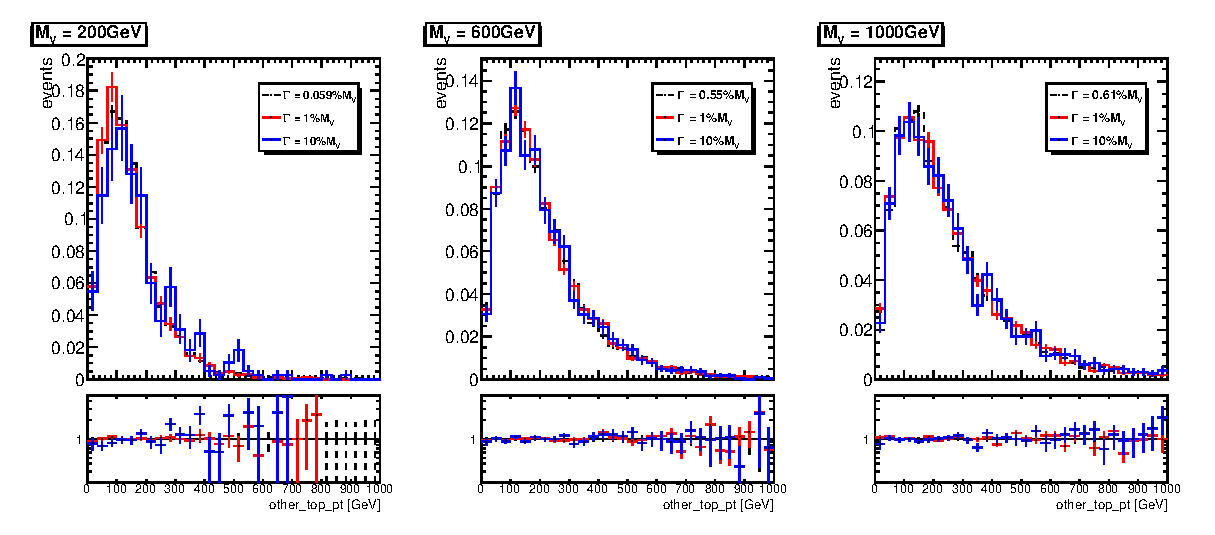
\includegraphics[width=1.0\textwidth]{figures/singletop/other_top_pt}
	\caption{
		Distribution of the top quark $p_T$ produced in association with $V$ in $gu\to tV$ for $m_V$ = {200, 600, 1000}~GeV (from left to right) and for three different
		visible decay width (computed from Madgraph directly, $1\%$ and $10\%$).
	}
	\label{fig:appB:pTtop}
\end{figure}

The limited timescale allowed to reach a consensus for
the recommendations contained in this document has not allowed further studies on the 
parameter scan of these models. The two Collaborations have however agreed to continue studying
these models and agree on a common parameter scan,
following the same path as for other models described in this document.  

%\newthought{Parameter choices and cross sections}
%
%\textbf{[Open point: update with new numbers]}
%
%ATLAS has considered two models, a resonant and a non-resonant production, using only right-handed top quarks in the lepton+jets final state. The signal samples were produced with {\sc Madgraph5} v1.5.11 interfaced with {\sc Pythia} 8.175, using the MSTW2008LO Parton Distribution Function (PDF) set (lhapdf ID: 21000).
%The mass of the top quark was set at 172.5 GeV. Dynamic renormalisation and factorisation scales were used.
%The $\met$ particle mass was varied, and in the case of the resonant model the resonance mass was fixed at 500~GeV:
%\begin{itemize}
%\item Resonant model,  $\met$ particle mass: [0,100]~GeV in 20~GeV steps
%\item Non-resonant model, $\met$ particle mass: [0,150]~GeV in 25~GeV steps, [200,300]~GeV in 50~GeV and [400,1000]~GeV in 100~GeV steps 
%\end{itemize}
%
%%\com{How to translate the monotop paper couplings to the notation of this note? }
%The couplings $\ares$ and $\anonres$ are set at a fixed value of $0.2$.
%In addition, two samples are produced for the resonant model for $\mfmet=100$~GeV,
%with coupling strengths fixed at $\ares=0.5$ and $\ares=1.0$,
%in order to check the effect of the resonance width on the signal event kinematics. 
%The total width of the resonance varies quadratically with the coupling strength,
%corresponding to a width of 3.5~GeV, 21.6~GeV, and 86.5~GeV at $\ares=0.2$, $\ares=0.5$, and $\ares=1.0$, respectively.
%
%The number of free parameters is reduced by assuming $(\ares^q)_{\mathrm{12}}=(\ares^q)_{\mathrm{21}}=(\ares^{1/2})_{\mathrm{3}}\equiv \ares$
%for the resonant model and $(\anonres)_{\mathrm{13}}=(\anonres)_{\mathrm{31}}\equiv \anonres$ for the non-resonant model,
%all other elements of these coupling matrices being equal to 0.
%For each model, the coupling parameter $\ares$ or $\anonres$ and the masses of the exotic particles are independent.
%
%The cross-sections as well as the width of the resonance for the resonance model are shown in Table~\ref{tab:S1R_Xsec}.  
%The cross-section is slowly decreasing when $m(f_{met})$ increases,
%and the values do not differ by larger than 10\%, due to the similarity of the kinematics, in the chosen mass range.
%\begin{table}[!htb]\centering
%\begin{tabular}{l|r|r|r}
%\hline \hline
%% $\mathrm{m}(f_{\mathrm{met}})$ [GeV] & $\sigma\times\mathrm{BR(S\rightarrow t f_{met})}\times\mathrm{BR(t\rightarrow l^+\nu b)[pb]}$ & $\sigma\times\mathrm{BR(S\rightarrow t f_{met})}\times\mathrm{BR(t\rightarrow jjj)[pb]}$ & $\Gamma(S)$ [GeV]   \\
%$m(f_{met})$ [GeV] & $\sigma_{lep}$~[pb] & $\sigma_{had}$~[pb] & $\Gamma(\Phi)$ [GeV]   \\
%\hline \hline
%0                        &  1.107              & 2.214               &  3.492  \\
%20                       &  1.102              & 2.205               &  3.491  \\
%40                       &  1.089              & 2.180               &  3.487  \\
%60                       &  1.068              & 2.137               &  3.481 \\	
%80                       &  1.039              & 2.078               &  3.472  \\
%100                      &  1.001              & 2.003               &  3.461  \\
%100 ($\ares=0.5$) &  6.091              &  12.13              & 21.63    \\
%100 ($\ares=1.0$  &  21.77              &  43.72              &  86.52   \\
%\hline \hline
%\end{tabular}
%\caption
%{
%Theoretical predictions for the product of the production cross-section of the
%scalar resonance, the branching ratio of its decay into a top quark and the invisible particle,
%and of the branching ratio of the top quark decay into a semi-leptonic ($\sigma_{lep}$) or fully-hadronic ($\sigma_{had}$) final state,
%in the resonance model.
%Values are given for a resonance of mass 500~GeV and for an effective coupling $\ares=0.2$ (except for two masses),
%as a function of the mass $m(f_{met})$ of the neutral fermion.
%The total widths $\Gamma(\Phi)$ of the resonance are also shown.
%}
%\label{tab:S1R_Xsec}
%\end{table}
%
%
%For the non-resonant case, the cross-sections are given in Table~\ref{tab:S4R_Xsec} and are calculated with $\anonres=0.2$.
%The cross-section diverges when $m(v_{met})$ tends to 0~GeV.  However, when the mass is exactly 0~GeV the cross-section has a finite value,
%due to the specificity of the propagator for this massless spin-1 boson.
%\begin{table}[!htb]\centering
%\begin{tabular}{l|r|r}
%\hline \hline
%% $m(v_{met})$ [GeV] & $\sigma\times\mathrm{BR(t\rightarrow l^+\nu b)[pb]}$ & $\sigma\times\mathrm{BR(t\rightarrow jjj)[pb]}$ \\
%$m(v_{met})$ [GeV] & $\sigma_{lep}$~[pb] & $\sigma_{had}$~[pb] \\
%\hline \hline
%0                  &  96.03              & 192.4    \\
%25                 &  359.0              & 717.9    \\
%50                 &  113.4              & 226.9    \\
%75                 &  59.86              & 119.5    \\
%100                &  37.45              & 74.82    \\
%125                &  25.35              & 50.68    \\
%150                &  18.00              & 35.96    \\
%200                &  9.662              & 19.28    \\
%250                &  5.506              & 11.02    \\
%300                &  3.328              & 6.656    \\
%400                &  1.372              & 2.738    \\
%500                &  0.6345             & 1.270    \\
%600                &  0.3192             & 0.6354   \\
%700                &  0.1698             & 0.3383   \\
%800                &  0.09417            & 0.1883   \\
%900                &  0.05472            & 0.1091   \\
%1000               &  0.03259            & 0.06479  \\
%\hline \hline
%\end{tabular}
%\caption
%{
%Theoretical predictions for the product of the production cross-section of the invisible vector $v_{met}$ and of a top quark,
%and of the branching ratio of the top quark decay into a semi-leptonic ($\sigma_{lep}$) or fully-hadronic ($\sigma_{had}$) final state, 
%in the non-resonance model.
%Values are given for an effective coupling $\anonres=0.2$, as a function of the mass $m(v_{met})$ of the invisible state.
%}
%\label{tab:S4R_Xsec}
%\end{table}

% \com{I think it might make more sense to have the joboption information in a public web site instead of
% adding all the details into the note. Reference only visible for ATLAS members: \\
% {\small https://svnweb.cern.ch/trac/atlasoff/browser/Generators/MC12JobOptions/trunk/gencontrol/MadGraphControl$\_$Monotop.py}}

%\textbf{[Open point: systematic uncertainties]}
% \com{Question for DM forum:
% \begin{itemize}
%  \item Do we want to give more details about the Madgraph implementation, the couplings value in the param\_card, etc ... ?
%  \item I am not aware of any work on systematic variation due to scale, PDF choice, showering (Maybe some was done in the monotop analysis?). Then I am not completely what to put here.
% \end{itemize}
% }



 
 \section{\texorpdfstring{Models with a single $b-$quark + MET}{Models with a single b-quark + MET}}
\label{sec:singleb}
 Models of bottom-flavored Dark Matter that are closely related to the $t-$channel mediated model from this 
Section have been proposed in Refs.~\cite{Lin:2013sca,Agrawal:2014una}. 
Here, DM couples preferentially to bottom quarks, with a decoupled third generation. 
We describe the $b$-FDM model of Ref.~\cite{Agrawal:2014una}, created to explain the Galactic Center (GC) 
gamma-ray excess observed in data collected by the Fermi-LAT collaboration~\cite{Daylan:2014rsa,Calore:2014xka}. 
This model favors couplings to third-generation quarks via Yukawa couplings, 
therefore respecting the MFV assumption. 

This model produces an annihilation cross section consistent with the gamma-ray excess
that has perturbative values for the couplings and is
consistent with LHC constraints on the colored mediator.
For parameters capable of explaining the anomalous gamma-ray signal in terms of Dark Matter 
coupling preferentially to $b$-quarks, the model predicts a direct detection cross section that is consistent 
with current constraints, but within the near future reach of Direct Detection experiments and of the
upcoming LHC run. 
%The model will be decisively tested with data from the upcoming high-energy run at the LHC. 

The model contains a Dirac fermion transforming as a flavor triplet, exclusively coupling
to right-handed down-type quarks. The third component of the triplet $\chi_b$ comprises the 
cosmological DM. Within the MFV framework, the other fermions in the flavor triplet can be 
made sufficiently heavy and weakly-coupled that they can be neglected in the analysis.
A flavor singlet, color triplet scalar field $\Phi$ mediates the interactions between the DM 
and the Standard Model quarks. The model is similar to the MSSM with a light bottom squark and neutralino, 
and is thus a flavor-specific example of a \tchannel model. 
\Todo{Spell out implications on MFV assumption, and whether top-flavored could exist too.}

The Lagrangian considered is given by
\begin{equation}
  -{\cal L} \supset g \Phi^* \bar\chi_b b_R  + {\rm h.c.}
\end{equation}

%The QCD production of the colored mediator introduces a tree-level $b$+MET diagram with a $g_s*g$ dependence, which could be scaled. 
%However, the bb+MET (which often also falls in the b+MET signal region) has both pure QCD production of the colored mediator 
%($g_s^2$) and also possibly diagrams that scale as $g_s^2*g$. 

\paragraph{Parameter scan}

The nature of the model is not conducive to a simple scaling behavior that would allow us to reduce the number of points to be simulated. This is because of the interference of diagrams with QCD production of the mediator (which scale as $g^2_s$) with diagrams that are proportional to the coupling $g$ in the $b+$\MET{} and $b\bar{b}$+\MET{} final states. Fixing the couplings also fixes the mediator width, when adopting the minimal width assumption. 

A full study of the parameter scan for this model was not available for this report; thus we recommend scanning a range of  possible widths as discussed in a more-limited way for the \schannel mono-jet, spanning from the minimal width to a value approaching the particle limit, e.g. $g=0.5,1,2,3$. A coupling benchmark such as $g=1$ should be considered for each mass point since this would be a distinctive feature of this benchmark from SUSY models with sbottom squarks (see Section~\ref{sec:monojet_t_channel} for further discussion): Cross-sections for unit couplings can be found in Appendix~\ref{app:xsecs_bFDM}. The coupling could also be chosen to fulfill constraints from the relic density (see Appendix~\ref{app:Relic_Density_bFDM}, with corresponding cross sections in Tables~\ref{tab:g_relic_13T} onwards). 

A scan of Dark Matter and mediator masses should be done in the on-shell region $M_\Phi > \mDM + m_b$, since the cross-sections in the off-shell region are too small to be sensitive with early LHC data, spanning from 10 to 500 GeV in \mDM and from 10 to 1300 GeV in \mMed. 

%  \item $\mDM=10-500$ GeV with a binning of 50 GeV for $\mDM<100$ and  100 GeV otherwise; 
%  \item $MPhi=10-1300$ with a binning of 100 GeV;

% Therefore, the coupling scan is chosen as a discrete set of values $g=0.5,1,2,3$ for each mass point.
%~\Todo{Are we sure the models in SVN have minimal width? What is the max coupling so that the width is still lower than the mass?}

\begin{figure}[h!]
    \begin{minipage}{0.49\textwidth}
      \centering 
      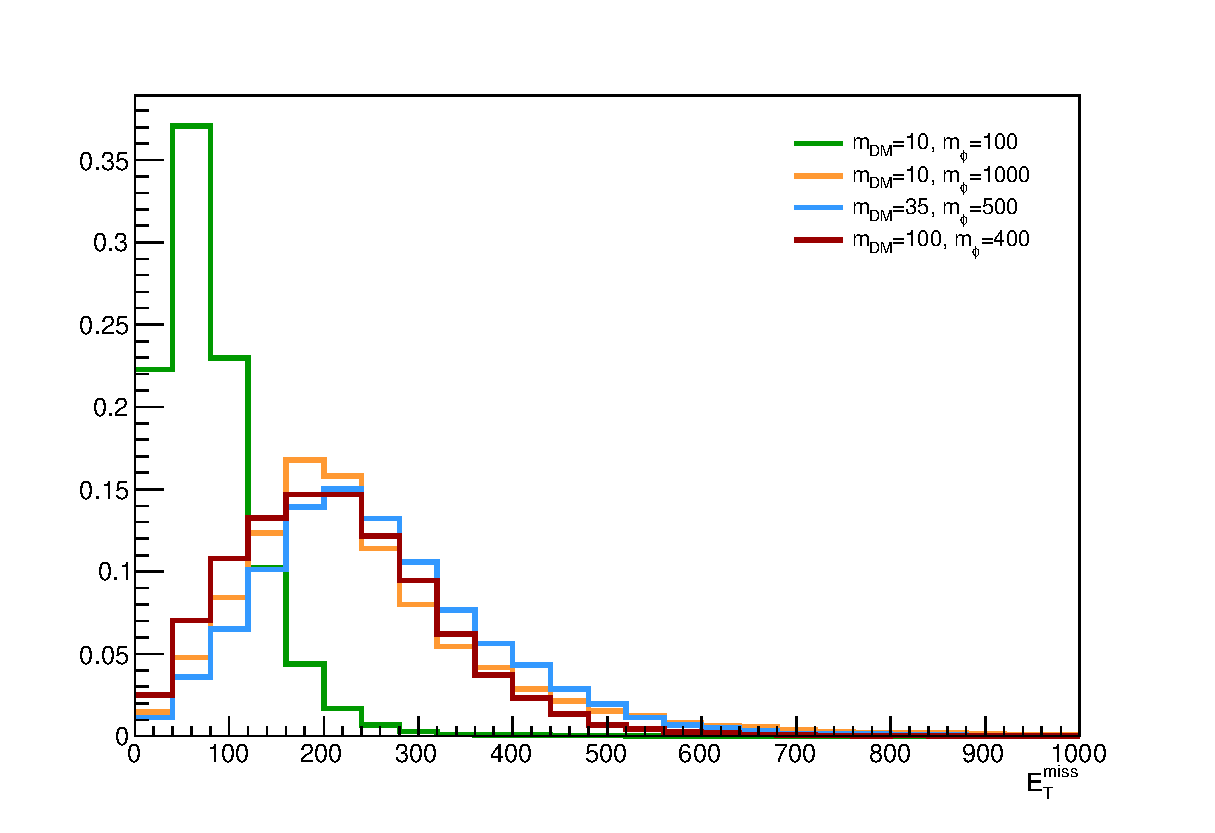
\includegraphics[scale=0.32]{figures/bFDM/bfdm_relic/missing_et.eps}
    \end{minipage}
    \hfill
    \begin{minipage}{0.49\textwidth}
      \centering 
      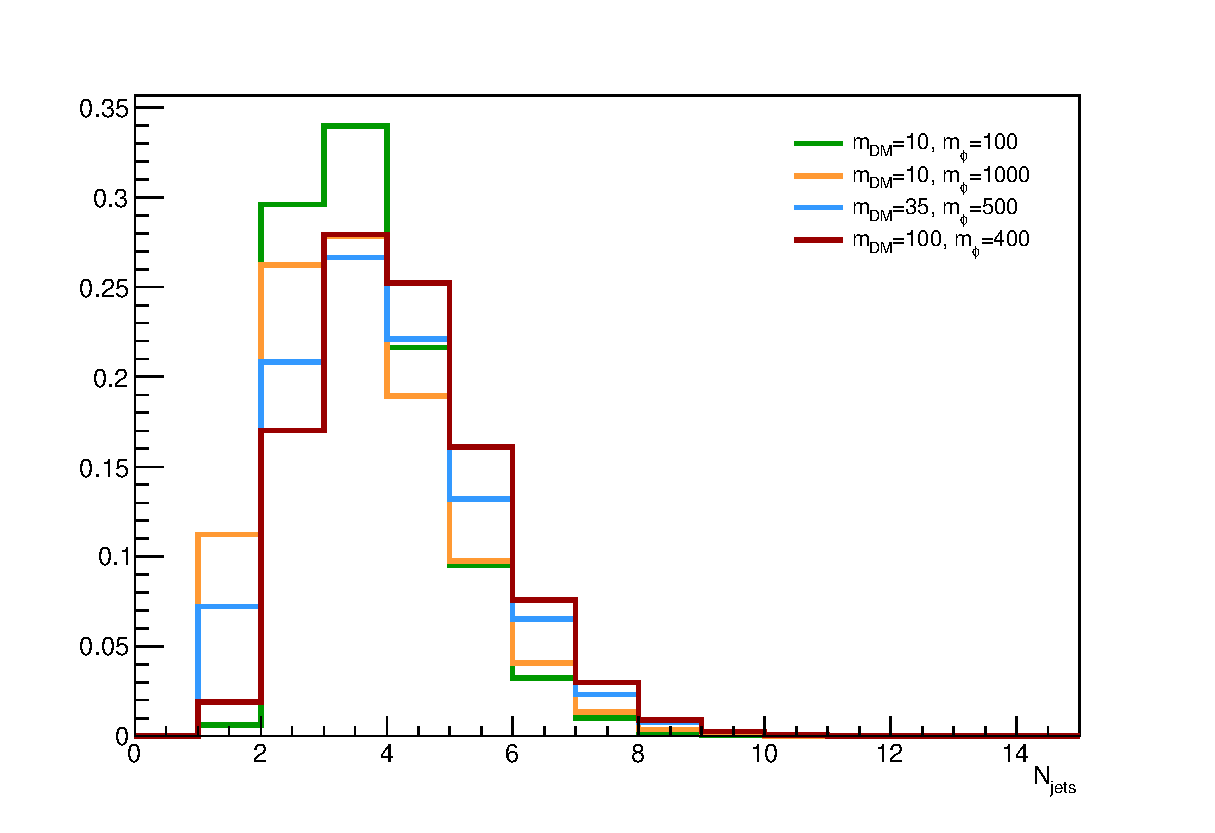
\includegraphics[scale=0.32]{figures/bFDM/bfdm_relic/Njets.eps}
    \end{minipage}
    \caption{MET (left) and jet multiplicity (right) for various DM and mediator masses and couplings normalized to the relic density observed in the early universe. \label{fig:relic}}
\end{figure}

\begin{figure}[h!]
    \begin{minipage}{0.49\textwidth}
      \centering 
      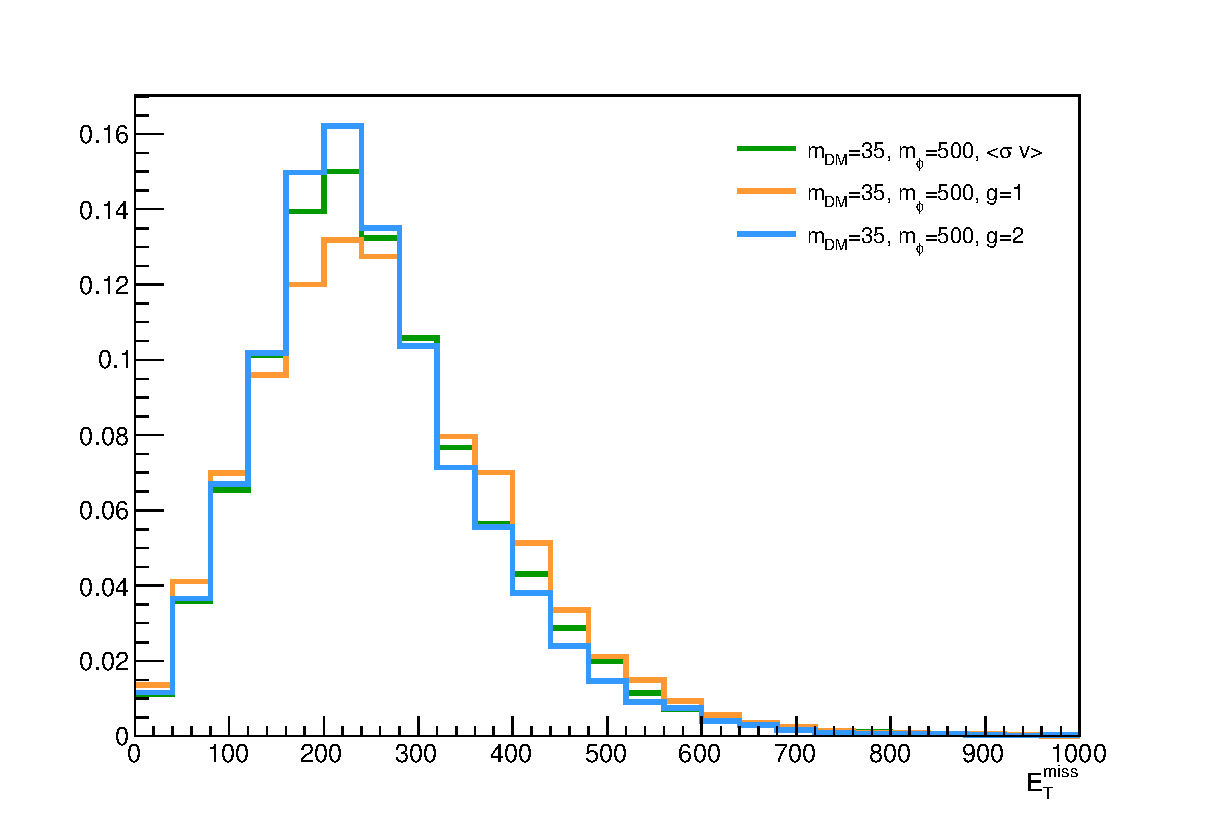
\includegraphics[scale=0.32]{figures/bFDM/bfdm_35_500/missing_et.eps}
    \end{minipage}
    \hfill
    \begin{minipage}{0.49\textwidth}
      \centering 
      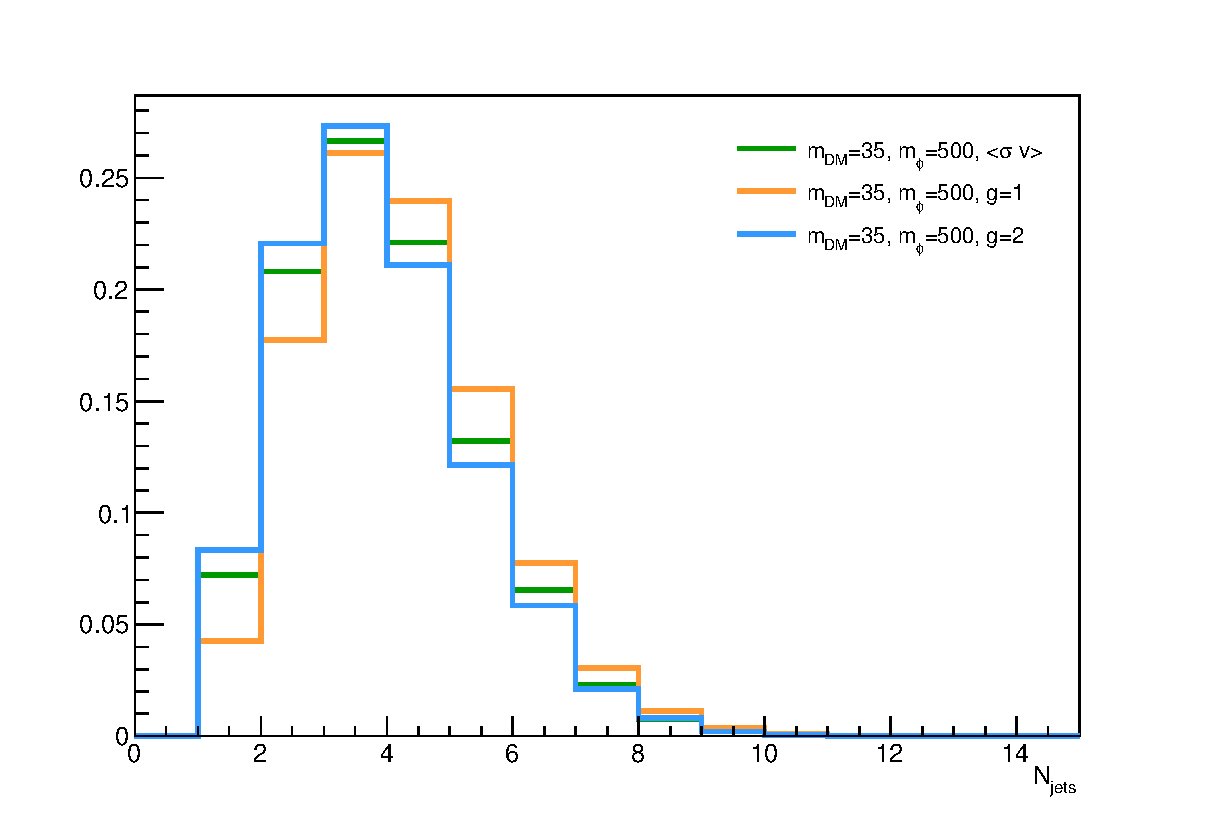
\includegraphics[scale=0.32]{figures/bFDM/bfdm_35_500/Njets.eps}
    \end{minipage}
    \caption{MET (left) and jet multiplicity (right) for $\mDM=35$~GeV and $MPhi=500$~GeV for couplings corresponding to relic density weights and also $g=1,2$ \label{fig:g_comp}}
\end{figure}

%The following benchmark points could be produced as a starting point for the parameter space for this model:
%
%\begin{itemize}
%  \item $\mDM=10-500$ GeV with a binning of 50 GeV for $\mDM<100$ and  100 GeV otherwise; 
%  \item $MPhi=10-1300$ with a binning of 100 GeV;
%  \item $MPhi > \mDM + m_b$, since the cross-sections in the off-shell region are too small to be sensitive with early LHC data;
%\end{itemize}

%This scan of the parameter space is summarized in Table~\ref{tab:monobscan}.
%
%\begin{table}[!h]
%\centering
%\resizebox{\textwidth}{!}{
%\begin{tabular}{| l |r r r r r r r r r r r r r r|}
%\hline
%\multicolumn{1}{|c|}{\mDM (\gev)} & \multicolumn{14}{c|}{\mmed (\gev)} \\
%\hline
%  10 &   10 &  100 &  200 &  300 &  400 &  500 &  600 &  700 &  800 &  900 & 1000 & 1100 & 1200 & 1300 \\
%  50 &      &  100 &  200 &  300 &  400 &  500 &  600 &  700 &  800 &  900 & 1000 & 1100 & 1200 & 1300 \\
% 100 &      &  100 &  200 &  300 &  400 &  500 &  600 &  700 &  800 &  900 & 1000 & 1100 & 1200 & 1300 \\
% 200 &      &      &  200 &  300 &  400 &  500 &  600 &  700 &  800 &  900 & 1000 & 1100 & 1200 & 1300 \\
% 300 &      &      &      &  300 &  400 &  500 &  600 &  700 &  800 &  900 & 1000 & 1100 & 1200 & 1300 \\
% 400 &      &      &      &      &  400 &  500 &  600 &  700 &  800 &  900 & 1000 & 1100 & 1200 & 1300 \\
% 500 &      &      &      &      &      &  500 &  600 &  700 &  800 &  900 & 1000 & 1100 & 1200 & 1300 \\
%\hline
%\end{tabular}
%}
%\caption{Simplified model benchmarks for the considered mono-$b$ model, as described in the text.}
%\label{tab:monobscan}
%\end{table}

%The increase in the center of mass energy from 8 to 13 TeV leads to a cross-section increase that is a function of $MPhi$, 
%with a smaller dependency for \mDM. Therefore, the sensitivity to this model will increase in early 13~TeV data compared to 8 TeV searches~\cite{Aad:2014vea}.



